\chapter{Arhitektura i dizajn sustava}
\paragraph{}{Web aplikacija je softverski program koja se izvršava na web poslužitelju i koja omogućuje korisnicima pristup i interakciju s raznim funkcijama, uslugama ili informacijama putem web preglednika.}
\begin{figure}[!htb]
	\centering
	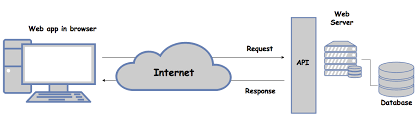
\includegraphics[width=1\linewidth]{dijagrami/arhWeb.png}
	\caption{ Arhitektura sustava}
	\label{fig:arhsustava}
\end{figure}
\paragraph{}{Povezanost između web aplikacije i web poslužitelja je ključna za funkcioniranje web aplikacija. Evo osnovne poveznice:}
\begin{packed_item}
		\item  \textbf{ Klijentska strana (Frontend):}
		\begin{packed_item}
			\item { Web aplikacija obično ima klijentsku stranu koja se izvršava u web pregledniku korisnika. Ova klijentska strana može biti izrađena korištenjem HTML-a, CSS-a i JavaScripta, a može koristiti i frontend okvire poput React-a kojeg smo odabrali u izradi naše web aplikacije.
			}
		\end{packed_item}
		\item  \textbf{Poslužiteljska strana (Backend):}
			\begin{packed_item}
			\item {Backend dio web aplikacije izvršava se na web poslužitelju. Ovdje se izvršava poslovna logika aplikacije, upravlja se bazom podataka, obrađuju se zahtjevi korisnika, provjerava se autentikacija, autorizacija itd. Backend se obično piše u jezicima poput Node.js, Pythona, Rubyja, Java-e, a mi smo se odlučili za C\verb|#| zajedno s .NET radnim okvirom.}
			\end{packed_item}
			\paragraph{}{}\paragraph{}{}
		\item  \textbf{ Komunikacija između klijenta i poslužitelja:}
		\begin{packed_item}
			\item {Web aplikacija komunicira s poslužiteljem putem HTTP (Hypertext Transfer Protocol) zahtjeva i odgovora. Kada korisnik interagira s web aplikacijom putem svog preglednika (klikne na gumb, ispuni obrazac), preglednik šalje zahtjev web poslužitelju. Web poslužitelj obrađuje taj zahtjev i šalje odgovor natrag pregledniku.
			}
		\end{packed_item}
		\item  \textbf{ Povratne informacije korisniku:
		}
		\begin{packed_item}
			\item {Kada web poslužitelj obradi zahtjev, šalje odgovor natrag na klijentsku stranu (preglednik). To može uključivati HTML, CSS, JavaScript, podatke iz baze podataka ili druge resurse koji se prikazuju korisniku putem web preglednika.
			}
		\end{packed_item}
		
\end{packed_item}
\paragraph{}{Odabrali smo Microsoft Visual Studio kao naše razvojno okruženje. Koristit ćemo arhitekturu sustava temeljenu na MVC (Model-View-Controller) konceptu. Ovaj koncept podržan je unutar .NET radnog okvira te pruža gotove predloške koji olakšavaju razvoj web aplikacija.
	Jedna od glavnih karakteristika MVC koncepta je njegova sposobnost za nezavisni razvoj pojedinih dijelova aplikacije. Ovo omogućuje lakše testiranje aplikacije kao i jednostavnije dodavanje novih svojstava u sustav bez potrebe za velikim modifikacijama.
}
\paragraph{}{MVC arhitektura se sastoji od:
}
 \begin{packed_enum}
	
	\item Model: Model predstavlja sloj podataka aplikacije i poslovnu logiku. Ovdje se podaci obrađuju, pohranjuju i pristupa im se. Model je odgovoran za interakciju s bazom podataka ili nekim drugim izvorom podataka, kao i za manipulaciju tim podacima prema zahtjevima poslovne logike.
	\item View: View predstavlja korisničko sučelje aplikacije, odnosno ono što korisnik vidi i s čime interagira. Pogled prikazuje podatke iz Modela na način koji je razumljiv i koristan korisniku. Obično se radi o HTML-u, CSS-u, JavaScriptu ili nekom drugom obliku sučelja koje korisnik može vidjeti.
	\item Controller: Kontroler je posrednik između Modela i View-a. On obrađuje korisničke zahtjeve primljene putem korisničkog sučelja (View), upravlja tim zahtjevima i ažurira Model prema tim zahtjevima. Kontroler reagira na akcije korisnika, ažurira podatke u Modelu i određuje koji View će se prikazati korisniku.
	
\end{packed_enum}
\section{Baza podataka}

\paragraph{}
{Za potrebe razvoja aplikacije SpotPicker koristi se relacijska baza podataka. 
Osnovne zadaće baze podataka su pohrana i organizacija podataka te brzo pretraživanje 
i dohvaćanje podataka kako bi ih se moglo dalje obraditi.
Svaki je entitet korištene relacijske baze naveden i opisan u daljnjem tekstu, 
a ispod opisa nalazi se tablični prikaz opisanog entiteta i njegovih atributa.}

\paragraph{}{Baza podataka aplikacije SpotPicker sastoji se od sljedećih entiteta:}
\begin{packed_item}
	\item ConfirmationLink
	\item Korisnik
	\item Parking
	\item Rezervacija
	\item Wallet
\end{packed_item}


\subsection{Opis tablica}

\paragraph{}
{\emph{ConfirmationLink}\\
Entitet ConfirmationLink sadrži informacije vezane za potvrđene korisnike i sadrži sljedeće atribute:
ConformationLinkID, KorisnikID, Link i isValid. Primarni ključ entiteta ConfirmationLink je atribut ConformationLinkID, a strani ključ je atribut KorisnikID.
Navedeni je entitet u vezi \emph{One-to-One} s entitetom Korisnik preko atributa KorisnikID.}

	\begin{longtblr}[
					label=none,
					entry=none
					]{
						width = \textwidth,
						colspec={|X[6,l]|X[6, l]|X[20, l]|}, 
						rowhead = 1,
					} %definicija širine tablice, širine stupaca, poravnanje i broja redaka naslova tablice
					\hline \SetCell[c=3]{c}{\textbf{ConfirmationLink}}	 \\ \hline[3pt]
					\SetCell{LightGreen}Confirmation LinkID & INT	&  	jedinstveni ID svakog linka sa potvrdu pri registraciji  	\\ \hline
					\SetCell{LightBlue} Korisnik ID	& INT & jedinstveni ID korisnika 	\\ \hline
					Link	& NVARCHAR &  točan link koji se koristio za potvrdu registracije	\\ \hline 
					isValid & BIT &  informacija o potvrdi korisnika \\ \hline  
	\end{longtblr}
\paragraph*{}
{\emph{Korisnik}\\
Entitet Korisnik sadrži informacije vezane za registrirane korisnike aplikacije i sadrži sljedeće atribute:
KorisnikID, Username, Password, RazinaPristupa, Name, Surname, PictureData, BankAccountNumber, Email, AccountEnabled i EmailVerified. 
Primarni ključ entiteta Korisnik je KorisnikID. 
Navedeni je entitet u vezi \emph{One-to-Many} s entitetom ConfirmationLink preko atributa KorisnikID, 
vezi \emph{One-to-Many} s entitetom Parking preko atributa KorisnikID, 
u vezi \emph{One-to-Many} s entitetom Rezervacija preko atributa KorisnikID 
i u vezi \emph{One-to-One} s entitetom Wallet preko atributa KorisnikID.}

	\begin{longtblr}[
					label=none,
					entry=none
					]{
						width = \textwidth,
						colspec={|X[6,l]|X[6, l]|X[20, l]|}, 
						rowhead = 1,
					} %definicija širine tablice, širine stupaca, poravnanje i broja redaka naslova tablice
					\hline \SetCell[c=3]{c}{\textbf{Korisnik}}	 \\ \hline[3pt]
					\SetCell{LightGreen}KorisnikID & INT	&  	jedinstveni ID korisnika  	\\ \hline
					Username	& NVARCHAR &  korisničko ime	\\ \hline 
					Password & NVARCHAR &  lozinka \\ \hline 
					Razina Pristupa & INT & voditelj parkinga(1) ili običan korisnik(0)	\\ \hline 
					Name	& VARCHAR &   ime korisnika	\\ \hline
					Surname	& VARCHAR &  prezime korisnika \\ \hline
					PictureData	& VARBINARY &   slika osobne	\\ \hline
					BankAccount Number	& VARCHAR &  broj bankovnog računa korisnika	\\ \hline
					Email	& VARCHAR &   korisnikova e-mail adresa	\\ \hline
					Account Enabled	& BIT &  informacija o potvrdi profila korisnika od strane administratora	\\ \hline
					Email Verified	& BIT &   informacija o potvrdi profila korisnika putem e-maila	\\ \hline
	\end{longtblr}
\paragraph{}
{\emph{Parking}\\
Entitet Parking sadrži informacije vezane za opis i konfiguraciju parkirališta te sadrži sljedeće atribute:
ParkingID koji je primarni ključ entiteta, Name, Description, Photo, PricePerHour, Capacity i KorisnikID. Strani ključ entiteta \emph{Parking} je KorisnikID.
Navedeni je entitet u vezi \emph{Many-to-One} s entitetom Korisnik preko atributa KorisnikID, 
i u vezi \emph{One-to-Many} s entitetom Rezervacija preko atributa ParkingID.
}

	\begin{longtblr}[
					label=none,
					entry=none
					]{
						width = \textwidth,
						colspec={|X[6,l]|X[6, l]|X[20, l]|}, 
						rowhead = 1,
					} %definicija širine tablice, širine stupaca, poravnanje i broja redaka naslova tablice
					\hline \SetCell[c=3]{c}{\textbf{Parking}}	 \\ \hline[3pt]
					\SetCell{LightGreen}ParkingID & INT	&  	jedinstveni ID parkirališta  	\\ \hline
					Name	& NVARCHAR &  naziv parkirališta	\\ \hline 
					Description & VARCHAR &  opis parkirališta \\ \hline 
					Photo & VARBINARY	&  	fotografija parkinga	\\ \hline 
					PricePerHour & INT	&  	cijena parkirališnog mjesta po satu	\\ \hline
					Capacity & INT	&  	broj parkirališnih mjesta na parkiralištu	\\ \hline
					\SetCell{LightBlue} KorisnikID	& INT &  jedinstveni ID korisnika	\\ \hline 
	\end{longtblr}	
\paragraph{}
{\emph{Rezervacija}\\
Entitet Rezervacija sadrži informacije vezane za rezervacije pojedinih parkirnih mjesta i sadrži sljedeće atribute:
ReservationID koji je primarni ključ entiteta, KorisnikID, ParkingID, DateTimeStart, DateTimeEnd i ParkingPlaceId. Strani ključevi entiteta \emph{Rezervacija} su KorisnikID i ParkingID.
Navedeni je entitet u vezi \emph{Many-to-One} s entitetom Korisnik preko atributa KorisnikID.
}

	\begin{longtblr}[
					label=none,
					entry=none
					]{
						width = \textwidth,
						colspec={|X[6,l]|X[6, l]|X[20, l]|}, 
						rowhead = 1,
					} %definicija širine tablice, širine stupaca, poravnanje i broja redaka naslova tablice
					\hline \SetCell[c=3]{c}{\textbf{Rezervacija}}	 \\ \hline[3pt]
					\SetCell{LightGreen} ReservationID & INT	&  	jedinstveni ID rezervacije  	\\ \hline
					\SetCell{LightBlue} KorisnikID	& INT &   jedinstveni ID korisnika	\\ \hline 
					\SetCell{LightBlue} ParkingID	& INT &  jedinstveni ID parkirališta 	\\ \hline 
					DateTimeStart	& DATETIME &  početno datum-vrijeme rezervacije  	\\ \hline 
					DateTimeEnd & DATETIME &  završno datum-vrijeme rezervacije \\ \hline 
					ParkingPlace ID & INT	&  	jedinstveni ID parkirališnog mjesta	\\ \hline 
	\end{longtblr} 
\paragraph{}
{\emph{Wallet}\\
Entitet Wallet sadrži informacije vezane za novčanik korisnika i njegova sredstva. Sadrži sljedeće atribute:
WalletID koji je primarni ključ entiteta, KorisnikID koji je strani ključ entiteta i Balance.
Navedeni je entitet u vezi \emph{One-to-One} s entitetom Korisnik preko atributa KorisnikID.
}

	\begin{longtblr}[
					label=none,
					entry=none
					]{
						width = \textwidth,
						colspec={|X[6,l]|X[6, l]|X[20, l]|}, 
						rowhead = 1,
					} %definicija širine tablice, širine stupaca, poravnanje i broja redaka naslova tablice
					\hline \SetCell[c=3]{c}{\textbf{Wallet}}	 \\ \hline[3pt]
					\SetCell{LightGreen}WalletID & INT	&  	jedinstveni ID novčanika  	\\ \hline
					\SetCell{LightBlue} KorisnikID	& INT &   jedinstveni ID korisnika	\\ \hline 
					Balance	& MONEY &   iznos sredstava u novčaniku korisnika	\\ \hline 
	\end{longtblr}


\subsection{Dijagram baze podataka}

\begin{figure}[!htb]
	\centering
	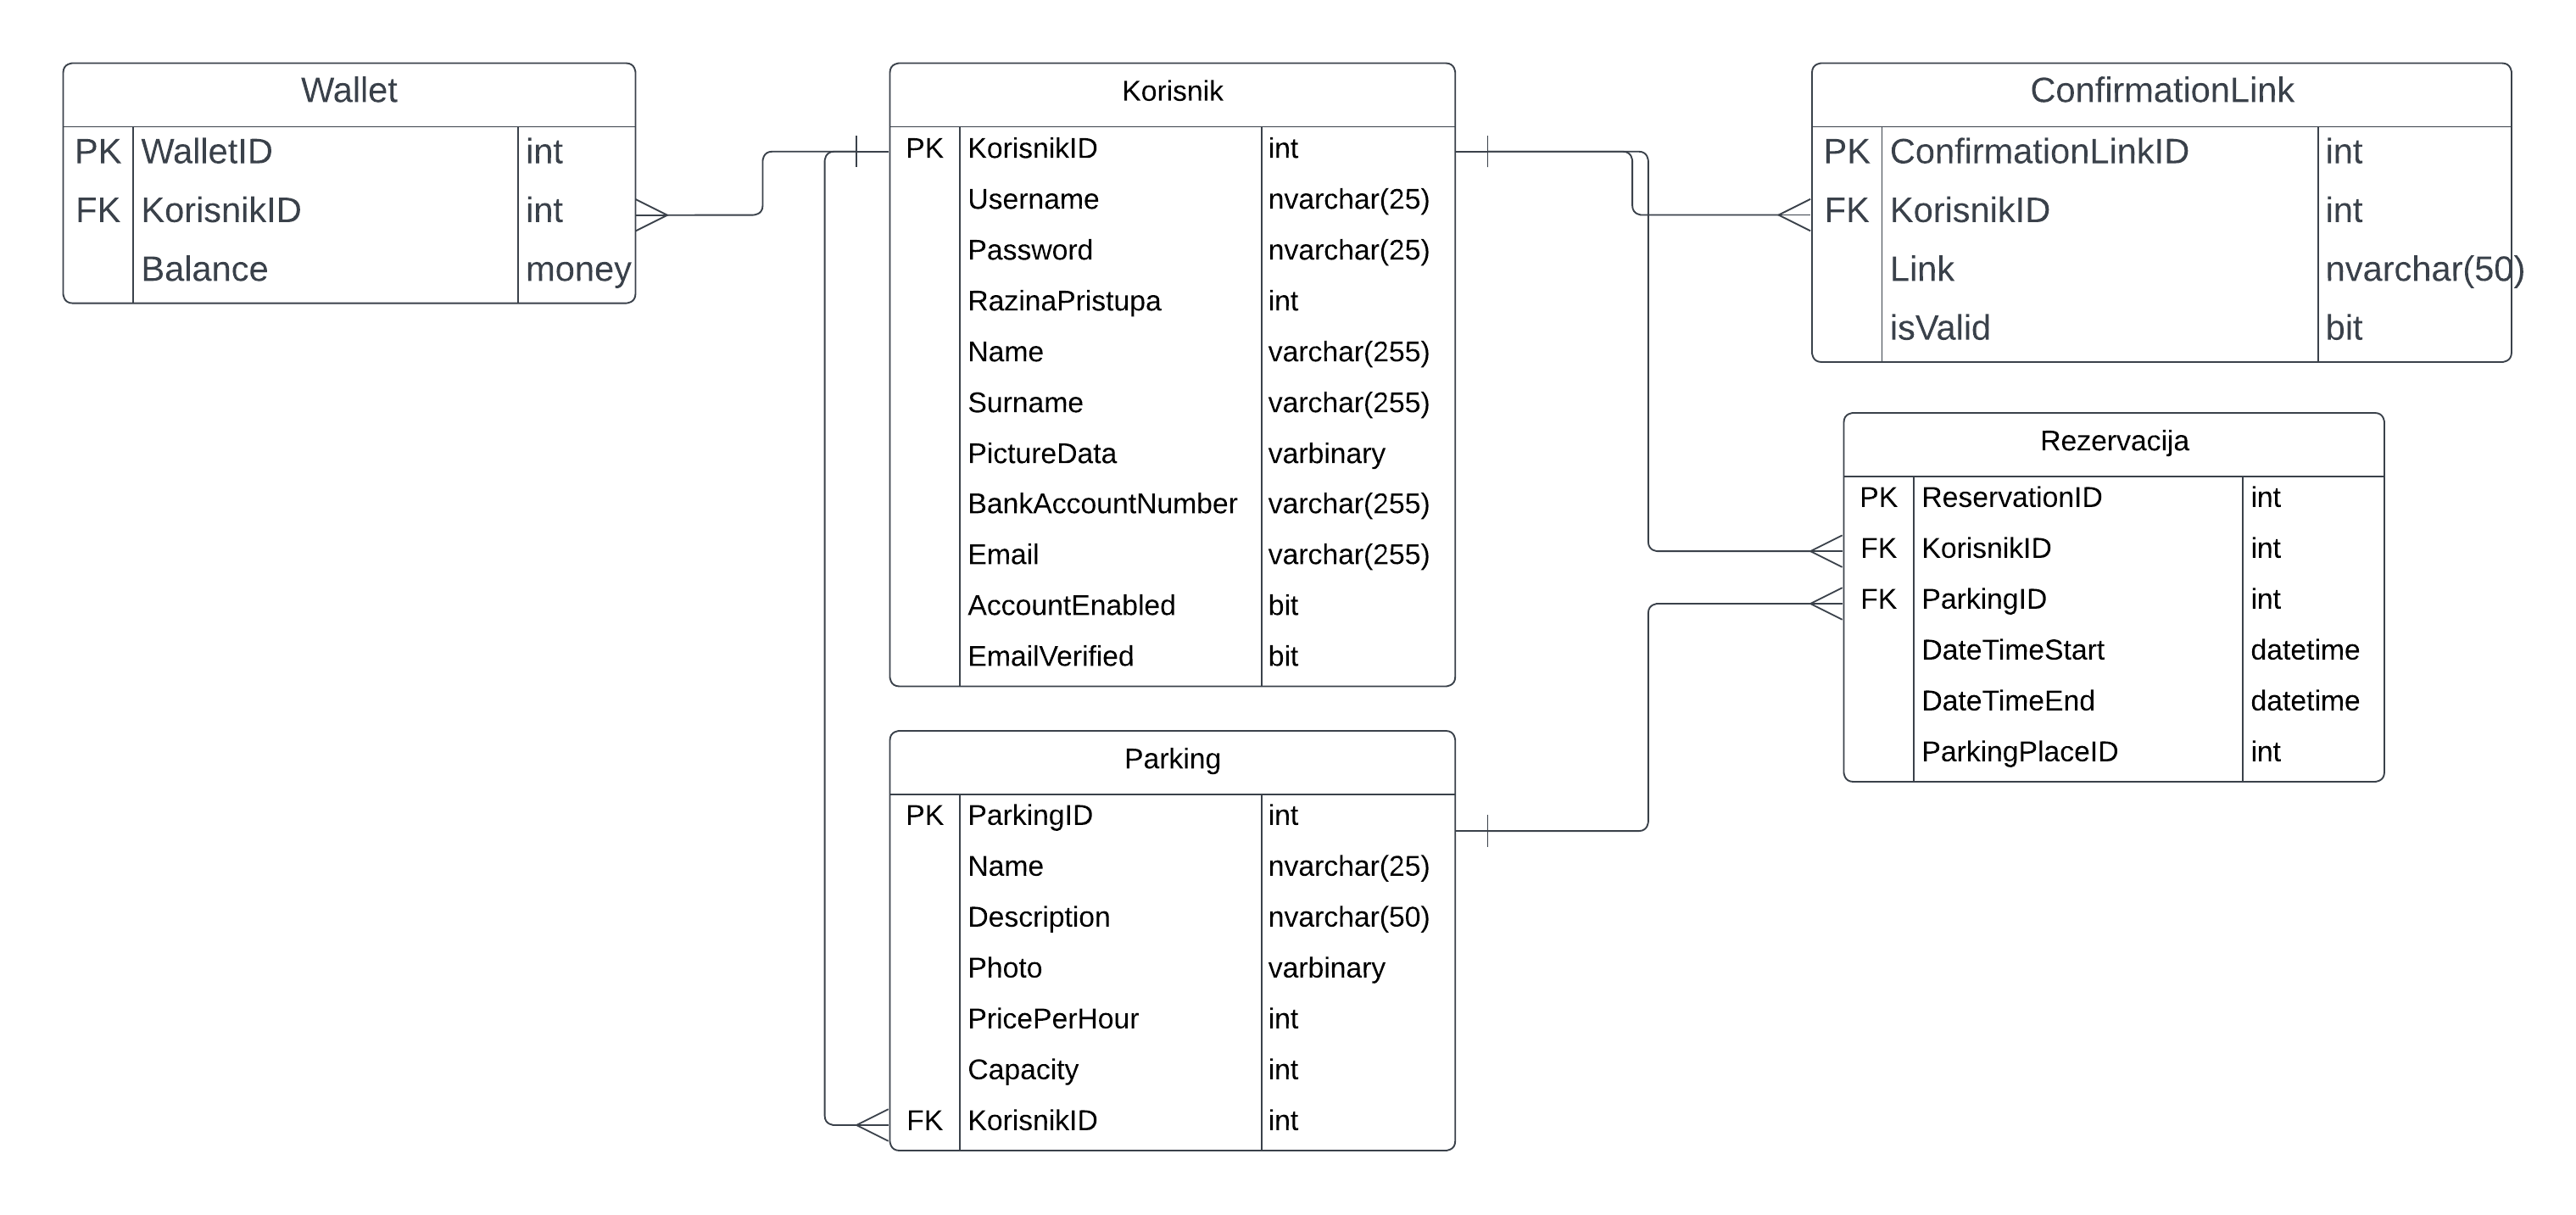
\includegraphics[width=1\linewidth]{dijagrami/ERdijagramPROGI.png}
	\caption{ ER dijagram baze podataka}
	\label{fig:dijagramklijent}
\end{figure}

\section{Dijagram razreda i opis razreda}

\paragraph{}
{Na slikama 4.3, 4.4 i 4.5 su prikazani razredi koji pripadaju \emph{backend} dijelu MVC
	arhitekture. Razredi prikazani na slici 4.3 nasljeduju Controller razred. Metode implementirane u tim razredima manipuliraju s DTO (Data transfer object), a oni su dohvaćeni pomoću metoda implementiranih u Model razredima. Metode implementirane u Controller razredima vraćaju JSON datoteke s html status kodom.
}
\vfill
\begin{figure}[!htb]
	\centering
	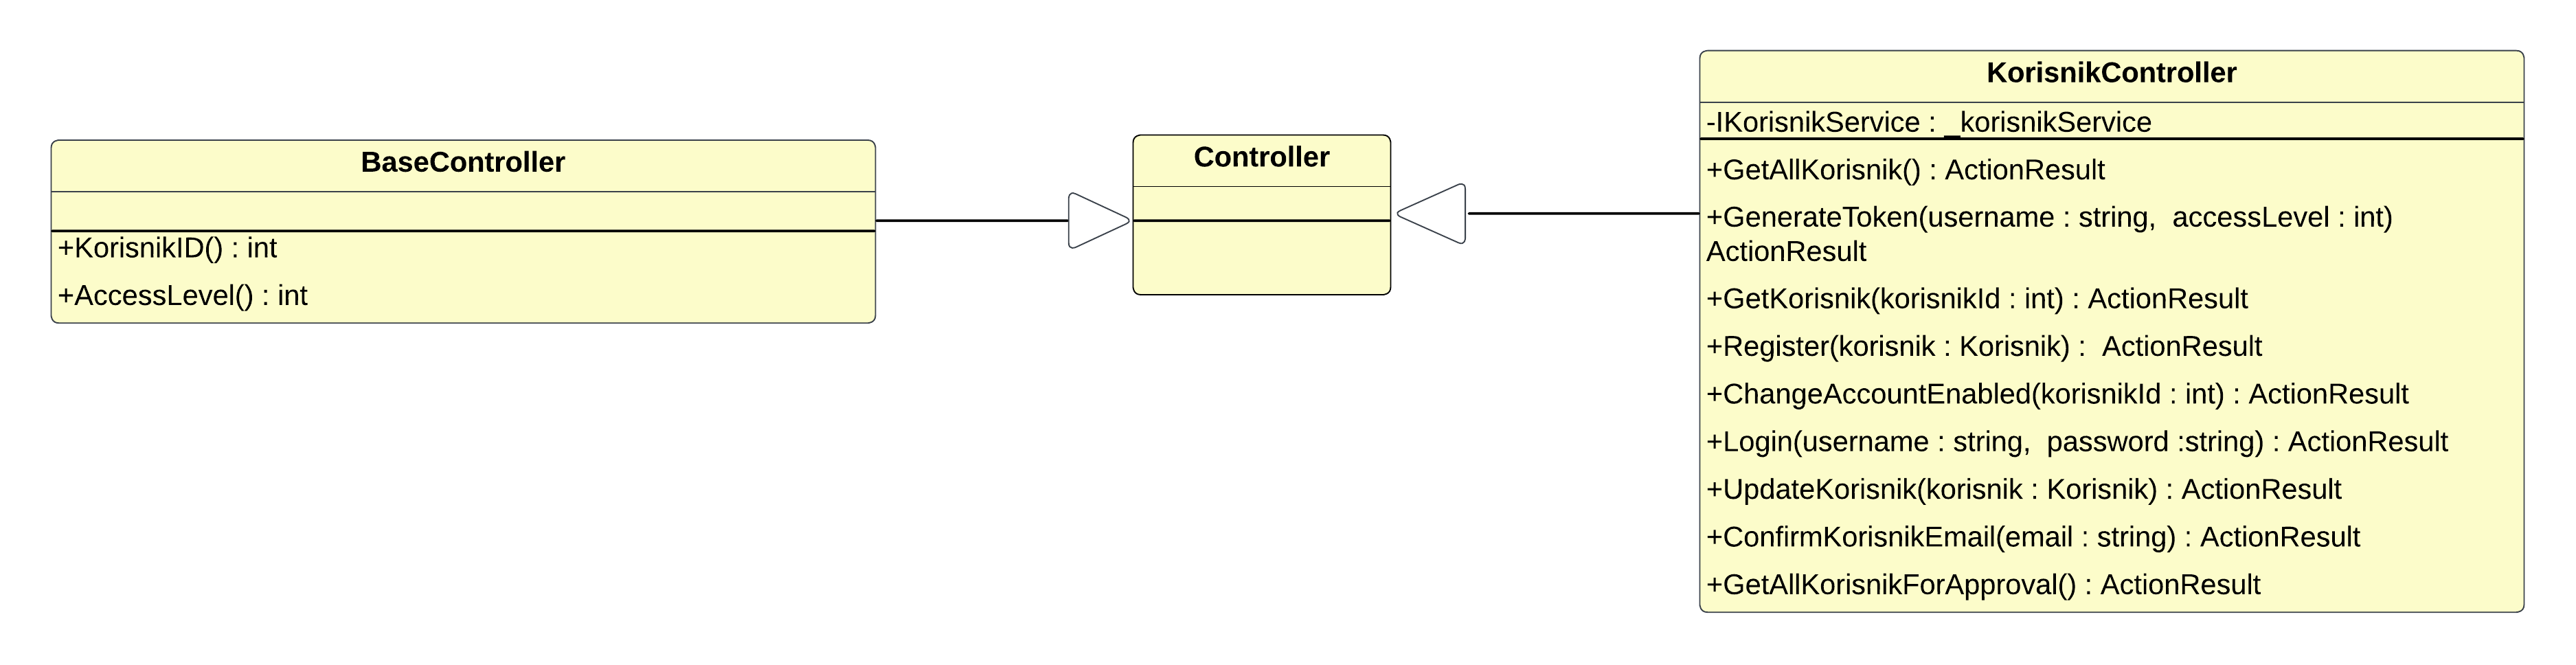
\includegraphics[width=1\linewidth]{dijagrami/ControllersDiagram.png}
	\caption{Dijagram razreda - dio Controllers}
	\label{fig:controllersdiagram}
	% Nakon \caption, stavite \vfill kako biste ostavili prazan prostor
	\vfill
\end{figure}

\begin{figure}[!htb]
	\centering
	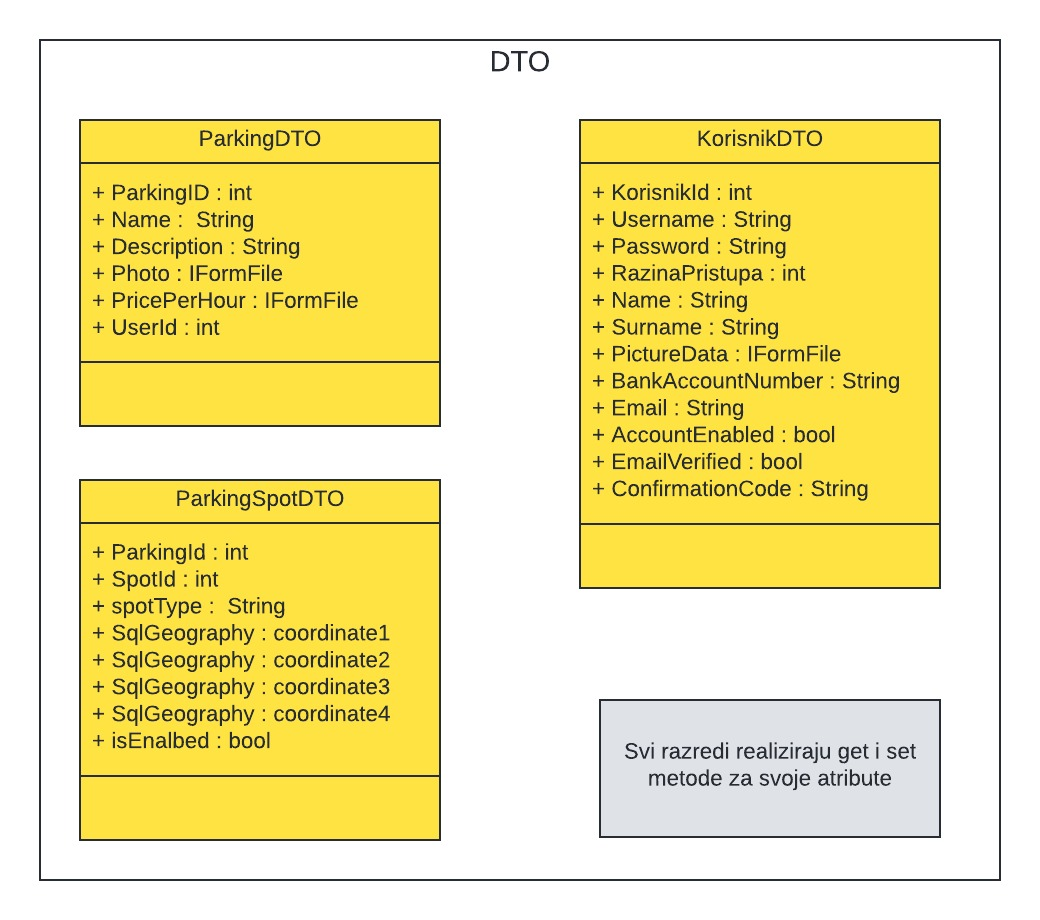
\includegraphics[width=1\linewidth]{dijagrami/DTODijagram.jpg}
	\caption{Dijagram razreda - dio Data transfer objects}
	\label{fig:dtodiagram}
	% Nakon \caption, stavite \vfill kako biste ostavili prazan prostor
	\vfill
\end{figure}

\paragraph{}
{Model razredi preslikavaju strukturu baze podataka u aplikaciji. Implementirane metode direktno komuniciraju s bazom podataka te vraćaju trazene podatke.
	Razred Korisnik predstavlja neregistriranog korisnika koji se moze registrirati u sustav kao klijent ili voditelj parkinga, unoseći osnovne informacije. Neregistrirani korisnik može vidjeti sva parkirna mjesta i posebno slobodna parkirna mjesta.
	Razred Klijent predstavlja korisnika koji je registriran u sustav. On moze koristiti osnovne funkcionalnosti sustava kao i neregistrirani korisnik i posebno dobiti informacije o zauzetosti pojedinih mjesta u stvarnom vremenu. Osim toga može nadoplatiti svoj novčanik i rezervirati parkirno mjesto.
	Razred Voditelj parkinga predstavlja registriranog korisnika koji može dodati parkirališta.
	Razred Administrator predstavlja administratora sustava koji ima najvece ovlasti. Ima mogućnost mijenjanja podataka registriranih korisnika i uklanjanje istih. Posebno potvrđuje voditelje parkirališta. 
	Razred Novčanik predstavlja novčanik klijenta te prikazuje iznos njegovih raspoloživih sredstava.
	Razred Parkiralište predstavlja parkiralište koje je dodao voditelj parkinga.
}



\begin{figure}[!htb]
	\centering
	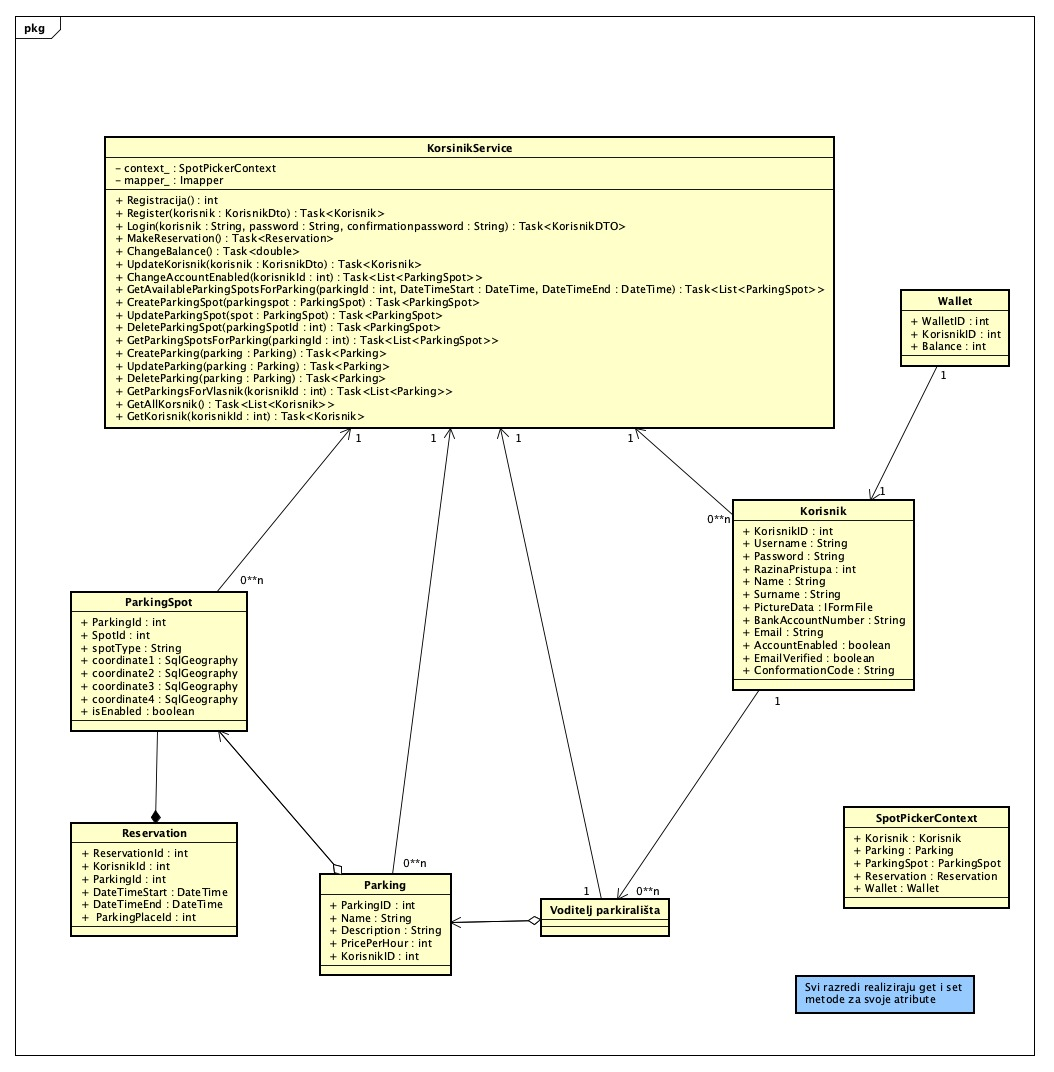
\includegraphics[width=1\linewidth]{dijagrami/SpotPickerModelsDiagram.png}
	\caption{Dijagram razreda - dio Models}
	\label{fig:modelsdiagram}
\end{figure}


\eject

\section{Dijagram stanja}

{Dijagram stanja za aplikaciju SpotPicker prikazuje moguća stanja korisnika i sustava te prijelaze između tih stanja na temelju različitih događaja. Na slici 4.6 prikazan je dijagram stanja za registriranog korisnika.
Nakon uspješne prijave u aplikaciju, registriranom korisniku se prikazuje početna stranica koja omogućuje pregled dostupnih parkirališta. Korisnik ima mogućnost pregleda informacija o svakom parkiralištu, njegovoj zauzetosti, te vrsti vozila koje se može parkirati. Za odabrano parkiralište korisnik može provjeriti informacije o cijenama, trajanju parkinga te dostupnim terminima za rezervaciju parkirališnih mjesta.
Korisniku je omogućeno nadopunjavanje novčanika putem aplikacije radi plaćanja rezervacija ili uplate parkinga prilikom dolaska na lokaciju slobodnog parkirališnog mjesta.}


% TODO: \usepackage{graphicx} required
\begin{figure}[!htb]
	\centering
	\includegraphics[width=1\linewidth]{dijagrami/STM - Registrirani Korisnik.jpg}
	\caption{ Dijagram stanja}
	\label{fig:dijagramstanja}
	
\end{figure}

\eject 